\documentclass{document_layout}
\usetikzlibrary{positioning}

% Title and author information 
\title{THERMOELECTRIC CONSIDERATIONS OF1
THREE-PHASE CONNECTIONS FOR SCHNEIDER
ELECTRIC}
\author{
    Eduardo Barroso\address{1}, Ariana Rodriguez\address{1} \\[0.5em]
    {\scriptsize
        \address{1} Department of Physics Engineering; Monterrey Institute of Technology, Monterrey, N.L 64849.\\
    }
}
\date{\today}

\setabstract{
    This work aims to provide an overview of simulations concerning the behavior of AC current carrying cables. The focus of the discussion is on the quasistatic limits of conducting matter and the analytic solutions derived for the field distributions within the cable. Additionally, the work delves into the examination of thermoelectric and mechanical stresses that are generated by the flow of currents through the cable. Through simulations, a comprehensive understanding of the intricate behaviors and effects of AC cables can be attained, aiding in the design and optimization of such systems for various applications.
}

% Begin the document
\begin{document}

\maketitle
    
\section{Introduction}
\label{sec:INTRO}
Precise and cost-efficient simulation of AC cable systems is crucial in modern electrical engineering. Fast and reliable simulation can improve the design and development process, allowing engineers to explore, evaluate and prototype more advanced and safe electrical wires. However, as these currents flow through cables, complex electromagnetic phenomena emerges such as skin effect, electromagnetic interference and proximity effect. Failing to understand the complex analysis required leads to costly or inaccurate simulations. 
\\

This work presents the theoretical implications of AC systems and implements accurate and cost-efficient simulation model. The analysis primarily revolves around three-phase alternating currents, commonly encountered in electrical systems, with the standard frequency of 60 Hertz and current values of 5,000 amperes. Results presented in this work are based on a single nuclei, copper wire with a caliber of 400 kcmil. In compliance with the guidelines outlined by the National Electric Code, the system is designed to accommodate a 5,000 ampere load using 15 cables.
\\

%%%%%%%%%%%%%%%%%%%%%%%%%%%%%%%%%%%%%%%%%%%%%%%%%%%%%%%%%%%%%%%%%%%%%%%%%%%%%%%%%%%%%%%%%%
\section{Variables}
To facilitate a comprehensive understanding of the model, the work presents a list of key variables that will be central to our analysis. Furthermore, thought sections \ref{sec:Conducting Matter and Currents} and \ref{sec:Quasistatic Fields} we will use the numerical values for such variables to present theoretical calculations. It is recommended to take a moment to familiarize with the critical variables. 
\\
\begin{table}[H]
\resizebox{\columnwidth}{!}{ % Scale to column width
\begin{tabularx}{\linewidth}{|c|c|X|}
\hline
\textbf{Name} & \textbf{Units} & \textbf{Value}\\
\hline
Current per cable ($I_0$) & [A] & 333.3 \\
\hline
Frequency ($w$) & [Hz] & $60 * (2\pi)$ \\
\hline
Radius (R) & [m] & 0.00897 \\
\hline
Length of cable & [m] & 1  \\
\hline
Electron mass ($m$) & [kg] & $9.1 * 10^{-31}$ \\
\hline
Electron charge ($q_e$) & [C] & $1.6021766 * 10^{-19}$ \\
\hline
Relaxation Time ($\tau$) & [s] & $2.48* 10^{-14}$ \\
\hline
Electron Density (n)& [$m^{-3}$] & $8.5 * 10^{28}$ \\
\hline
Conductivity ($\sigma$) & [$(\Omega m)^{-1}$] & $5.95*10^7$ \\
\hline
Permittivity ($\varepsilon$) &[F/m] & $ 1.476 * 10^{-6}$ \\
\hline
Permittivity free space ($\varepsilon_0$) & [F/m] & $8.8541878128 * 10^{-12}$ \\
\hline
Permeability ($\mu$) & [H/m] & $4\pi*10^{-7}$ \\
\hline
\end{tabularx}
} % Close fit
\caption{Critical Variables. This table presents key parameters related to copper conductors used in the study. The units specified for each parameter are shown in square brackets. }
\end{table}

The variables of permittivity and relaxation time are calculated with Drude's model of conductivity at low frequencies ($w < 10^{11}$) with no loss of generality. Furthermore, in section \ref{sec:RESULTS} the reader is presented with the calculations that take into account the experimental value of conductivity. This is done in order to ensure the accuracy and precision of the model. However, before diving into the details, the work proceeds to explain some basic notions to get all readers into context.
\\




\section{Conducting Matter and Currents}
\label{sec:Conducting Matter and Currents}
%%%%%%%%%%%%%%%%%%%%%%%%%%%%%%%
\subsection{Conducting Matter}
A perfect conductor is a macroscopic model for real conducting materials, characterized by the property that static electric fields are completely excluded from its interior. This means that inside a perfect conductor, the electric field is zero, and any charge present is distributed uniformly on the surface of the conductor. The Maxwell equation that underlies this phenomena is Gauss's Law, which relates the divergence of the electric field $E$ to the volumetric charge density $\rho$ via
\begin{equation}
\nabla \cdot E_{in}(r) = \frac{\rho(r)}{\epsilon_0},
\end{equation}
where  $\epsilon_0$ is the permittivity of free space and $\rho(r)$ has units of charge per unit volume. 
\\

Within the volume of the perfect conductor, Gauss's Law shows that the electric field and the charge density must be
\begin{equation}
\label{eq:gausslawconductors}
E_{in}(r) = \rho(r) = 0.
\end{equation}
In fact, this definition ensures that all excess charge accumulates on the surface as surface charge density. Cavendish originally proposed this idea: In the presence of an external field $E_{ext}$  the Coulomb forces rearranges charges inside the metal until the condition in equation \ref{eq:gausslawconductors} is satisfied. This is called polarization and in the general case and \textbf{electrostatic induction} when applied to conductors. 
\begin{figure}[H]
    \centering
    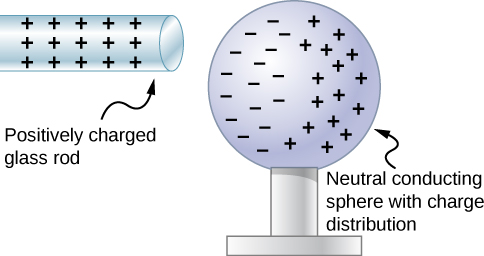
\includegraphics[scale=0.75]{Figures/electricpolarization.jpg}
    \caption{Polarized glass rod and electrostatic induction in sphere.}
    \label{fig:my_label}
\end{figure}

Physicists understand that in the metal, $\rho$ is associated with the electron's quantum mechanical wave functions which spread out over all available atoms. The force density $\rho E_{ext}$ disorts wave functions as to make charges with opposite signs displace in opposite directions \cite{zangwill2013modern}.


\subsection{Currents}
Current continuity equation underlies the conservation of electric charge in current related systems. Mathematically, this equation represents the relationship between current density $j$, and the flow of charge density $\rho$. It is expressed as
\begin{equation}
    \label{eq:continuity}
    \frac{\partial \rho}{\partial t} + \nabla \cdot j = 0, 
\end{equation}
and is derived from Maxwell's equations and plays a crucial role in understanding and analyzing the behavior of electric currents.
\\

In the context of direct currents, charge densities do not change in time so $\nabla \cdot j = 0$. Furthermore, these types of currents create time independent magnetic fields. Thus, the fields of interest satisfy conventional equations of electrostatics which lead to simple, accurate and cheap simulations\footnote{These are good attributes that underlie efficient and use full simulations}.
\\

Current density obey Ohm´s law in the static and time harmonic regime. Such law relates currents to the electric field and the conductivity $\sigma$ by
\begin{equation}
    \label{eq:ohmlaw}
    j = \sigma E.
\end{equation}
This result will be derived in the following section for the time harmonic condition. However, in direct current conditions it is easy to arrive starting from the familiar version of Ohm law
\begin{equation*}
    V=IR=jAR \rightarrow  j = (V/R)/A = \sigma E .
\end{equation*}
You just need to remember that conductivity is the inverse of resistivity and that voltage is related to the electric field. 
\\

\subsection{Drude's Classical Model}
Studying conductivity from a classical point of view provides a very clear physical picture of the phenomena as well as analytical expressions that describe the movement of electrons in conductors! Electron movement is described by a velocity $v(t)$ which is an average measure of how electrons drift through the metal´s atomic lattice and its commonly referred to as \textbf{drift velocity}. This velocity can be related to current and to conductivity as explained in the following paragraphs. 
\\

Start by considering $n$ electrons per unit volume where each one has a charge $q$ and mass $m$. When the conductor is connected to a AC voltage source it generates a time -harmonic electric field $\xi(r,t) = E(r)*exp(-iwt)$ inside the lattice resulting in a time harmonic current. Picture the electron traveling in the crystal structure of a metal (Figure \ref{fig:copper-structure}); the free electrons will eventually collide with atoms in the structure. The mean time of movement before  electrons suffer momentum-degrading collision is called \textbf{relaxation time} $\tau$ \cite{zangwill2013modern}. 
\begin{figure}[H]
    \centering
    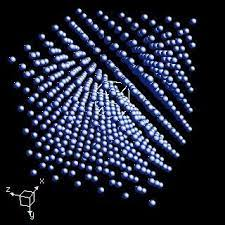
\includegraphics[scale = 0.5]{Figures/copper_structure.jpeg}
    \caption{Copper Crystalline Structure}
    \label{fig:copper-structure}
\end{figure}

Now, pay close attention. Newton´s force laws state that the force on the electrons is given by 
\begin{equation}
    m\frac{dv(t)}{dt}= q * E(r)*e^{-iwt} - \frac{mv(t)}{\tau} \hspace{0.5 cm}[N].
\end{equation}
Time harmonic solutions yield an expression for $v$ of the form
\begin{equation}
    v(t) = \frac{qE/m}{1/\tau -iw} e^{-iwt} = v(w)e^{-iwt} \hspace{0.5 cm}[m/s].
\end{equation}

Current density is formally defined in SI units with $[A/m^2]=[C/m^2s]$. It is simple to see that current density $j$ that develops in the system is given by
\begin{equation}
    \label{eq:current density distribution}
    j(w) = nqv(w) = \frac{nq^2 \tau}{m}\frac{E}{1-iwt} \hspace{0.3 cm}[A/m^2].
\end{equation}
\\

Result in \ref{eq:current density distribution} is then compared to \ref{eq:ohmlaw} to obtain \textbf{Drude´s model of conductivity} where
\begin{equation}
\label{eq:conductivity}
    \sigma(w) = \frac{nq^2 \tau/m}{1-iw\tau} = \frac{\sigma_0}{1-iw\tau} \hspace{0.5 cm}[S/m], 
\end{equation}
is identified as the conductivity of the material; closely related to the current density by Ohm´s law $ j(w) = \sigma(w) E(w)$. As the book \cite{jackson1999classical}, points out, quantum mechanical calculations give the same form for $\sigma$ for simple metals like copper.
\\

\subsection{Regarding Permittivity of Metal}
Permitivity of metal is desscribed by a complex magnitude and should be considered carefully in order to test the validity of crucial aproximations well encounter ahead. 
\cite{jackson1999classical}, continues the discussion by introducing the plasma frequency of the particulhttps://www.overleaf.com/projectar metal, $w_p ^2 = nq^2/\epsilon_0m$ and substuting \ref{eq:conductivity} into (err.find.zanwill.(18.12).  to derive Drude dielectric function,
\begin{equation}
\label{eq:Drude dielectric function}
    \epsilon(w) / \epsilon_0 = [1-\frac{w_p^2 \tau^2}{1+w^2\tau^2}]+i[\frac{w_p^2\tau}{w}\frac{1}{1+w^2\tau^2}]
\end{equation}

\subsection{Regarding Heat effects in currents}
To close this section on conductors with currents, it is worth wile mentioning that current is a process that changes kinetic energy of electrons into heat.  From the first law of thermodynamics (dU = Q-W = 0), the rate of joule heating is equal to the rate at which electric fields does work on the electrons. This phenomena of heat in cables is called joule´s law and is summarized
\begin{equation}
    \frac{dW}{dt} = \frac{d}{dt} \sum q_i E \cdot r = \int d^3r \nabla \cdot (j\phi) = RI^2,
\end{equation}
witch is used when considering thermo-electric effects in cables. 

\section{Dynamical Nature of Fields in AC currents}
\label{sec:Quasistatic Fields}
%%%%%%%%%%%%%%%%%%%%%%%%%%%%%
\subsection{Dynamic and Quasi-Static Fields}
The physics becomes more complex when considering alternating currents (AC). Recall, these currents are a consequence of the harmonics of the electromagnetic field where its constituents; the electric and magnetic fields are coupled to each other. For instance, a changing magnetic field is a source of electric fields and vice versa. Indeed, Maxwell´s equation dictate the coupling between changing electromagnetic fields. 
\\

Illustrated in section \ref{sec:Conducting Matter and Currents}, Maxwell's equations are the starting point of all electromagnetic phenomena \footnote{From electrical engineering to the physical origin of light.}. Having said this, we start by considering all the possible electromagnetic properties of matter, we proceed to build the equations that govern our cable system discarding properties only with physical arguments. This process will illustrate how the critical variables arise from theory and why.   
\\

Consider the total charge $\rho= \rho_f - \nabla \cdot P$ distinguishing free charge from polarization charge respectively. Similarly, the total current $j = j_f + \nabla \times M + \frac{\partial P}{\partial t}$, can be expressed as the sum of all possible contributions to current. Substituting these values into Maxwell´s equations and and defining auxiliary fields $D=\epsilon_0 E + P$ and $H = B/\mu_0 -M$ lead to Maxwell´s equations in matter
\begin{equation}
\begin{aligned}
    \begin{array}{cc}
    \nabla \cdot \mathbf{D} = \rho_f & \nabla \cdot \mathbf{B} = 0 \\
    \nabla \times \mathbf{E} = -\frac{\partial \mathbf{B}}{\partial t} & \nabla \times \mathbf{H} = \mathbf{j_f} + \frac{\partial \mathbf{D}}{\partial t}.
    \end{array}
\end{aligned}
\end{equation}

These laws describe the phenomenon's of electromagnetic induction and displacement currents. However, when considering the quasistatic limit where the sources change slowly enough in time to justify dropping one or the other of the time derivatives from the Maxwell equations. If the source is a slowly varying charge density $\rho(r,t)$ we neglect $dB/dt$ we have the quasi-electrostatic approximation. It applies to poor conductors since charge relaxation is slow. In contrast, when the source is a slowly varying current density $j(r, t)$, we neglect $dE/dt$ to get a quasi-magnetostatic approximation. This applies to good conductors where charge relaxation is fast and current frequency is low. \\

It is pertinent to add that experiments confirm that Coulumb-Lorentz force remains valid when sources and fields vary in time. This result will lead to generate a full analysis on forces arround cables. Recall that the general form of electromagnetic forces is given by
\begin{equation}
    \label{eq:force}
    F(t) = \int d^3r [\rho(r,t) E(r,t) + j(r,t) \times B(r,t)].
\end{equation}

\subsection{Quasi-Magnetostatics}
The following section aims to explain the three conditions that justify the use of this theory. First, we introduce the conditions and their meaning to latter present calculations obtained from the numerical evaluation applied in the context of metals like copper and aluminium. Pay close attention,
\\

Charge disappears from the bulk of good conductors faster than for a poor conductor. Thus, to a good approximation, we may set $\rho_f = 0$ and   $\nabla\cdot j_f = 0$. The latter is the steady-current condition that follows from the continuity equation \ref{eq:continuity}. 
\\
To find the quasistatic approximation note that the current density $ j_f = \sigma E $ in an Ohmic system is driven by an external source. Thus, we write Ampere-Maxwell
\begin{equation}
    \nabla \times B = \mu j_{ext} +\mu \sigma E + \mu \epsilon \frac{\partial E}{\partial t},
\end{equation}
 and calculate the contribution of displacement current density ($j_D = \mu \epsilon \partial E / \partial t$) \footnote{Writing $\nabla \propto 1/l$ and $d/dt \propto 1/T \propto w$.} by obtaining the following ratios
\begin{align}
\label{eq:quasimagnetostatic-condition}
\frac{j_D}{j_{\text{ext}}} &\propto \mu \epsilon w^2 l^2 \ll 1 \\
\frac{j_D}{j_f} &\propto \frac{\epsilon w E}{\sigma E} \propto w\tau_E \ll 1 \quad (\tau_E=\frac{\epsilon}{\sigma}).
\end{align}
 
When both conditions are satisfied, we have quasi-magneto-static behavior in conducting material \footnote{In the context of cables, l is the radius of the cable.}. More formally, since the contributions of the displacement current density are small, neglecting displacement current from Ampere-Maxwell law is valid. 
\\  %Por ahi de los 631 DRUDE

The physics in this regime depend on the relative importance of external vs induced fields. For example a field $B_{ext}$ produced by $j_{ext}$ create a Faraday electric field ($E_F \propto wl B_ext$). The corresponding current density $j_F = \sigma E_F$ produces its own Ampere magnetic field $B_F = \mu \sigma l E_F$. Therefore, if
\begin{equation}
\label{eq:inductioncondition}
    B_F/B_{ext} \propto \mu \sigma wl^2 = w\tau_m,
\end{equation}
we can build a the general quasi static condition as $(w\tau_M )(w\tau_E )<<1$. In other words, if $w\tau_m<<1$ electromagnetic induction is negligible and if its larger than one electromagnetic induction dominates.
\\
This theory is important because it is a quantitative justification the quasi-magnetostatic approximation. Formally, we modify Maxwell's laws in matter to obtain
\begin{equation}
\label{eq:MaxwellQuasiMagnetostatic}
    \begin{array}{cc}
        \nabla \times B = \mu \sigma E   &  \nabla \times E = - dB/dt.
    \end{array} 
\end{equation}
We can now justify this static approximation whenever $j_{ext}$ is negligible and when the current has low frequencies\footnote{The standard 60 Hz lies safely in the domain of quasi-magnetostatics. Zanwill continues to state that \ref{eq:quasimagnetostatic-condition} is satisfied up to ultraviolet frequencies ($10^17$ Hz) for high-conductivity materials like metals\cite{zangwill2013modern}.}. Furthermore, condition \ref{eq:inductioncondition} will tell us if induction effects dominate in our system.

\section{Mathematical Model}
\label{sec:RESULTS}

This following section aims to explain the thermo-electromagnetic phenomena underlying the simulation. Turns out, when considering the proper symmetries the simulations can be reduced in computation significantly \footnote{One of the critical success criteria.}.
\\

In the context of a straight cylindrical copper wire that carries a alternating current at standard frequencies, we consider the values at the tables to obtain $\epsilon = 1.4765 * 10^{-6}$, with
\begin{equation}
    w_p = \frac{nq^2}{\epsilon_0 m} = 1.645* 10^{16} [\frac{C^2 \Omega}{ m^2 s kg}],
\end{equation}
being the plasma frequency. Recall this frequency is used to calculate $\epsilon $ from Drude's dielectric function summarized by equation (9).
\\
Most importantly we must check quasi-magnetostatic conditions are met. Submitting our values to the conditions stated in equations \ref{eq:MaxwellQuasiMagnetostatic}, we obtain
\begin{equation*}
    \frac{j_D}{j_{ext}} =  \mu\epsilon w  R^2 = 2.1*10^{-11} << 1
\end{equation*}
when one considers no external currents, this condition is instantly met. For the latter and most important condition, we have
\begin{equation*}
     \frac{j_D}{j_{f}} = \frac{\epsilon w}{\sigma} = w \tau_E = \frac{\epsilon(w_p)*w}{\sigma}= 9.3*10^{-12} << 1,
\end{equation*}
in the code (annex 1) is found as \textsc{condition 2} and it is calculated with the values in the table in section II. \\

With both conditions met, it is secure to adopt the quasi-magnetostatic approximation with an accuracy of 99 percent. Furthermore, \cite{zangwill2013modern} shows that it is possible to derive the wave equation that governs the cable from Maxwell equations in the quasi-magnetostatic approximation \ref{eq:MaxwellQuasiMagnetostatic} obtaining:
\begin{equation}
    \nabla ^2 E =  \mu \sigma \frac{\partial E}{\partial t}.
\end{equation}

Assuming AC harmonic current $I(t)=I_0 e^{-iwt}$ allow us to propose the following anzatz $\xi(r,t)=E(r) \Psi(t)$. Furthermore, analysis in cylindrical coordinates $(\rho,\theta,z)$ has two symmetries in $\theta$ and $z$ that we'll exploit. This gives rise to a second-order ordinary differently equation describing the electromagnetic fields inside the cable 
\begin{equation}
\label{eq:diff-eqq-cylindrical}
    \rho \frac{\partial}{\partial \rho} (\rho \frac{\partial E}{\partial \rho}) + \kappa^2 \rho^2 E = 0 .
\end{equation}
Where the variable $\kappa = \sqrt{i\mu\sigma w} = (1+i)/\delta$ is closely related to the skin depth. Moreover, solutions to the former differential have the Bessel functions: $J_0(\kappa\rho)$ and $J_1(\kappa\rho)$; Related by Ampere-Maxwell in equation \ref{eq:MaxwellQuasiMagnetostatic}. Numerical field simulation can be implemented in the two dimensional transversal cut and dependent only on the radial variable $\rho$. If the cable is oriented in the $z$ direction, it is possible to define the fields
\begin{equation}
    E(\rho, t) = \Vec{z}  A J_0(\kappa \rho) exp(-iwt),
\end{equation}
and
\begin{equation}
    B(\rho, t) =  \Vec{\theta} \hspace{ 0.1cm} \frac{\kappa \rho}{iw} J_1(\kappa \rho) exp(-iwt).
\end{equation}
\\
Visualizing the behavior of the latter expressions we obtain the following figure
\begin{figure}[H]
    \centering
    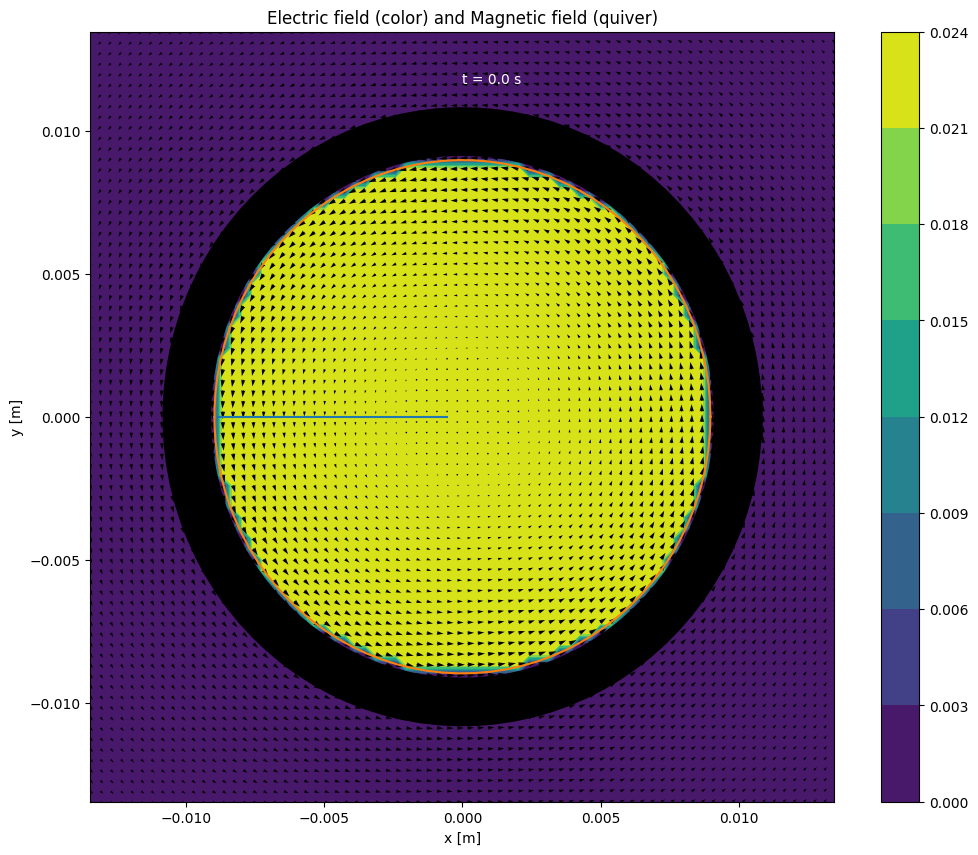
\includegraphics[scale=0.35]{Figures/em-fields-cable.png}
    \caption{Electromagnetic Field Visualization. Color represents electric field intensity and the quiver represents the magnetic field.}
    \label{fig:emfields-colorquiver}
\end{figure}

Furthermore, analyzing the behavior with respect to the radial distance we observe that the electric field has stronger values in the surface, explaining the skin effect. The magnetic field is also interesting because it illustrates the boundary conditions relating the inner and outer fields. 
\begin{figure}[H]
    \centering
    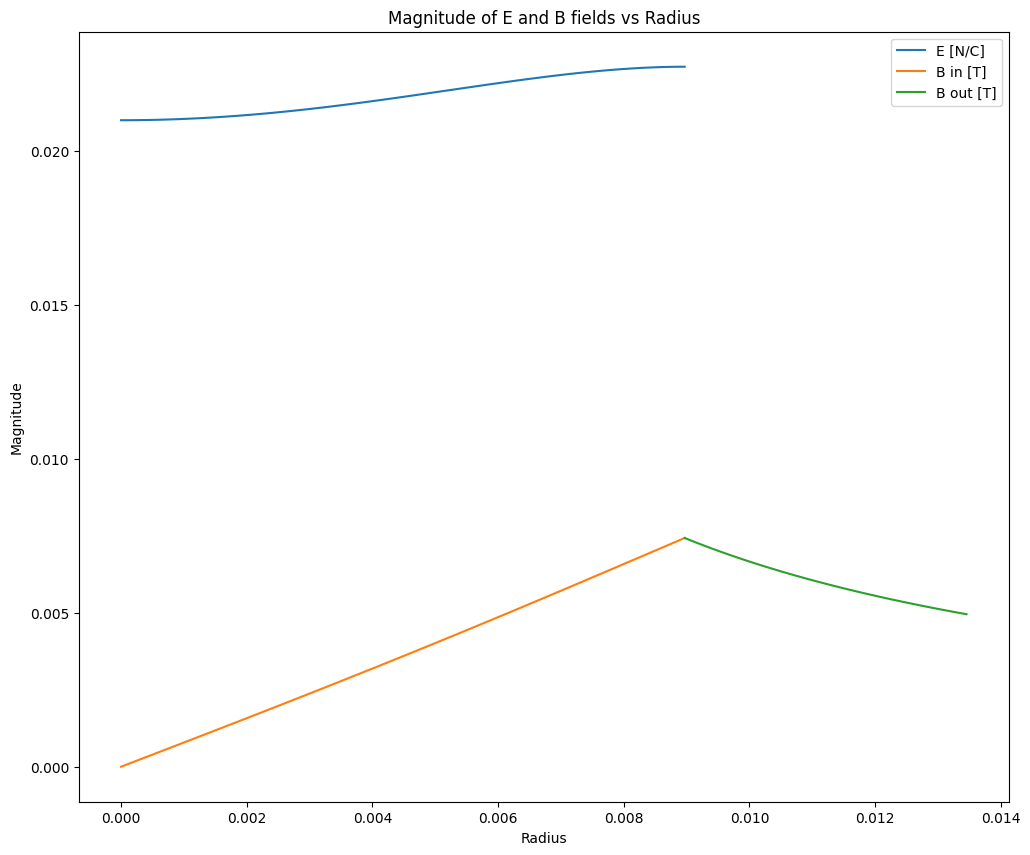
\includegraphics[scale=0.35]{Figures/magnitude-EvsB-radius.png}
    \caption{Electromagnetic fields as a function of radius.}
    \label{fig:emfields-radius}
\end{figure}

\subsection{The physics explaining the energy of the fields}
With these fields you can take two alternatives to calculate energy dissipation with poynting's vector and with the work energy of the electron-field interaction \footnote{Recall from such analysis, Joule´s rule was derived.}. The work proceeds to analyze the former and then the latter. 
\\
Poynting's vector is defined by Jackson \cite{jackson1999classical} as
\begin{equation}
    S = \frac{1}{\mu} E \times B \hspace{0.2cm} [\frac{J}{m^2s}].
\end{equation}
Particularly, we are interested on this vectors value at the surface since the flux of energy as heat is happening at the surface of the cable. The power $P = S* A$ is related to the heat energy $Q = P*t$, where area is determined by the cable parameters and the time is a single period of the AC oscillation. The results are presented in the figures bellow
\begin{figure}[H]
    \centering
    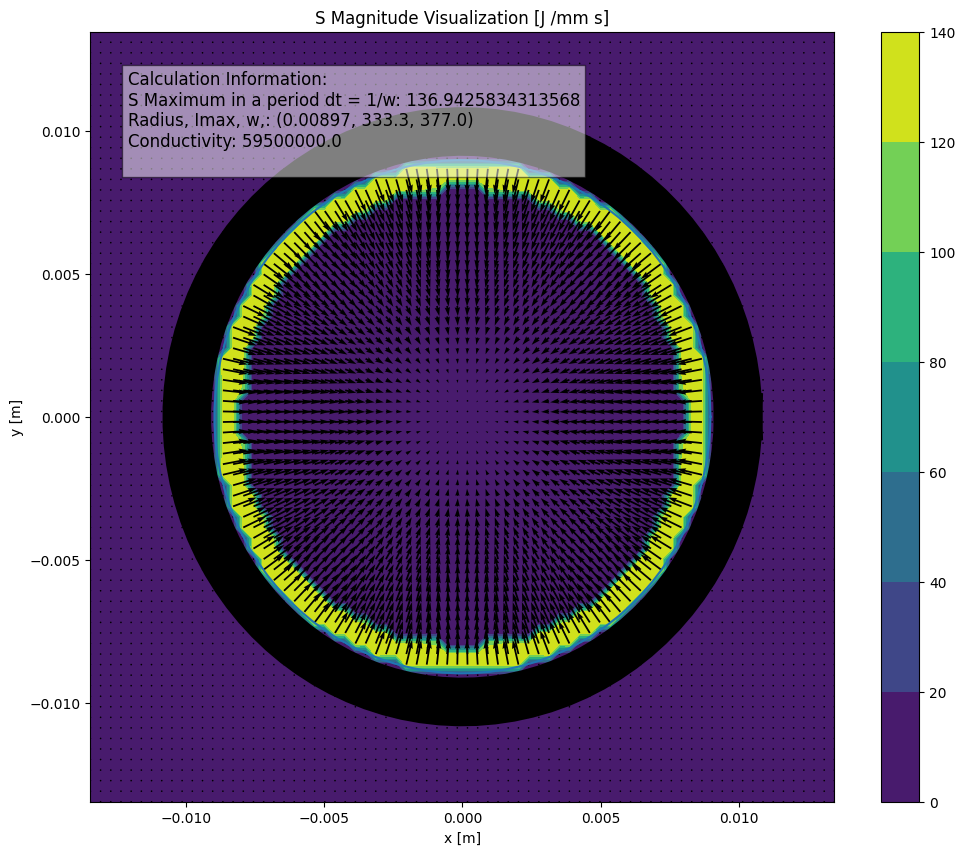
\includegraphics[scale=0.35]{Figures/poyinting-vector-cable.png}
    \caption{Poynting's Vector Visualization}
    \label{fig:poynting-colorquiver}
\end{figure}

For practical purposes, it is only necessary to arrive at Poynting's vector value. In fact, thermal simulation software calculate temperature distribution in a system given this value. For example, SolidWorks (R) only asks for poyntings value over the surface of the cable to calculate temperature. This reduces computation because in the case of more advanced software like ANSYS, the computer needs to solve Maxwells equations in all space and then solve the thermal or mechanical equations using finite element analysis. This work shows that is it possible to reduce the fist step of computation.
\\
For the sake of completeness, we present the power calculations in the following figure.
\begin{figure}[H]
    \centering
    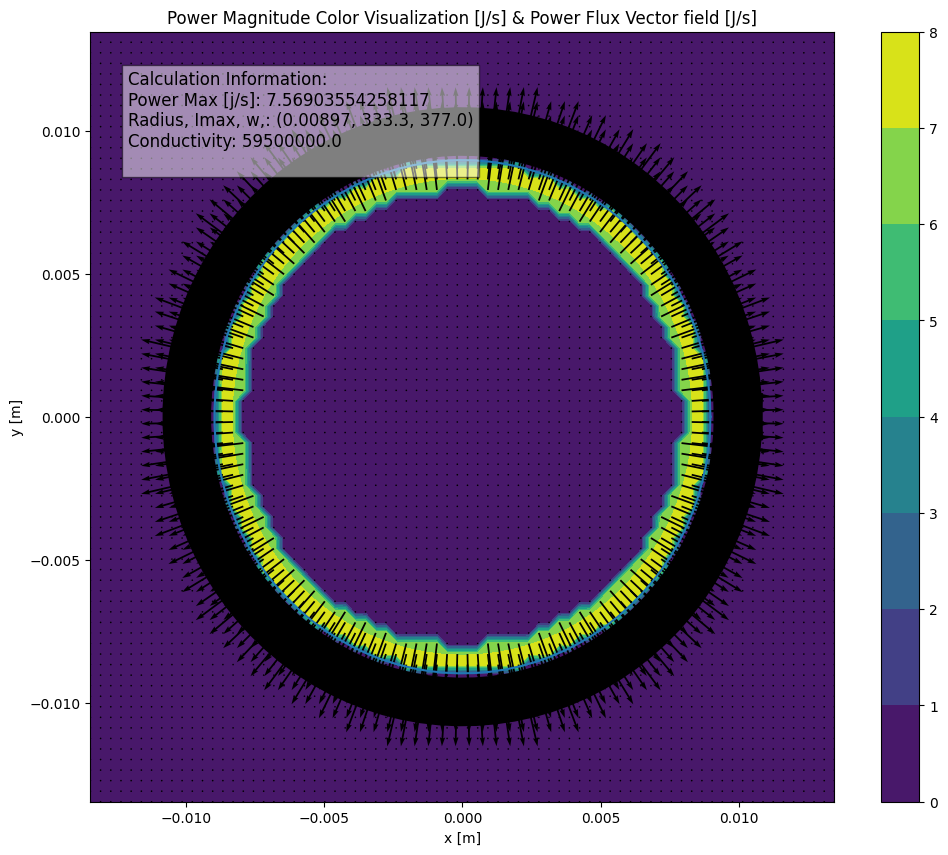
\includegraphics[scale=0.35]{Figures/power-q-cable.png}
    \caption{Power Visualization}
    \label{fig:power-colorquiver}
\end{figure}
As shown, the maximum power in purely electromagnetic calculations is 7.569 [W] while a the quick formula for Joule's rule yields 7.386 [W]. This difference can be explained due to the nature of both calculations. However, according to the modern theory of electrodynamics the power is greater than Joule's rule simplification. Therefore, using Joules rule can lead to problems because it gives lower heat fluxes than theory predicts.

\subsection{Skin effect}
Equation \ref{eq:diff-eqq-cylindrical} is related to the induction condition expressed in \ref{eq:inductioncondition} leading to the understanding how skin depth relates to induction via: $B_F/B_ext = \mu \sigma w R^2 = 2*R^2 / \delta^2$. Evaluating this condition in the system proposed we have $2.226 > 1$. The result hints at the fact that small induction will be present on our system. Moreover, relationship introduced above yields an expression for the skin depth of the form
\begin{equation}
    \delta(w) = \sqrt{\frac{2 }{\mu \sigma w}}.
\end{equation}
The former equation is the distance in meters from the surface into the core of the cable shown in figure \ref{fig:emfields-colorquiver}. The value obtained for the system under study is $\delta(w) = 0.00842$; just below the value of the nuclei radius $R$. This value is expected because condition \ref{eq:inductioncondition} expects small inductions.

\subsection{The physics underlying Joule's rule}
Notice that when considering Ohmic matter $j = \sigma E$ we can easily visualize the current density. Obtaining the current distribution is of great importance in order to validate our results. To understand why, we need to dive into the thermodynamics of the problem. \\
\begin{figure}[H]
    \centering
    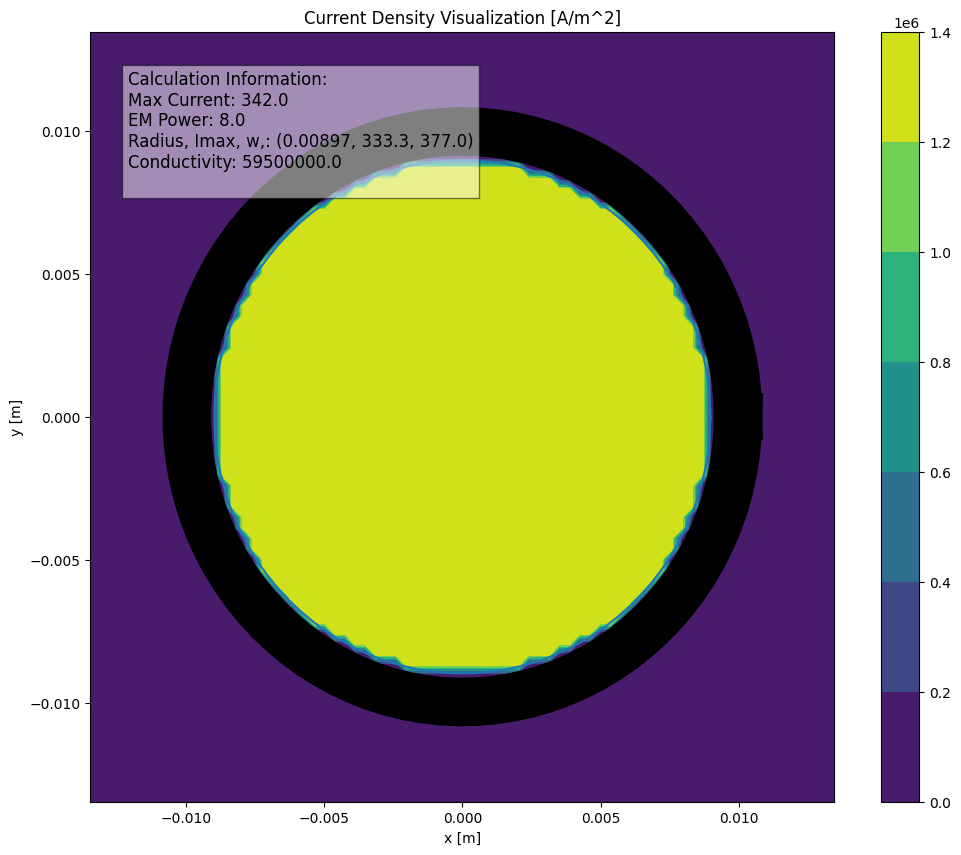
\includegraphics[scale=0.35]{Figures/current-density-cable.png}
    \caption{Current density Visualization}
    \label{fig:current-color}
\end{figure}
\begin{figure}[H]
    \centering
    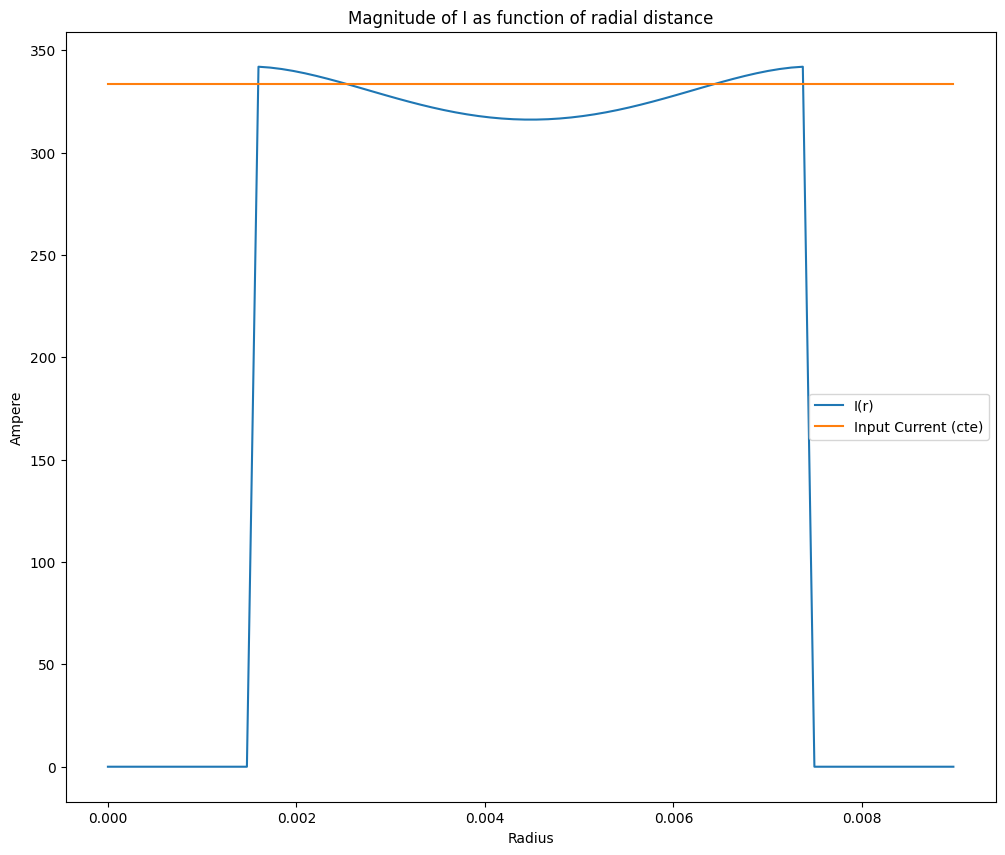
\includegraphics[scale=0.35]{Figures/magnitude-current-radius.png}
    \caption{Current Magnitude as a function of radius}
    \label{fig:current-color}
\end{figure}


Recall the first law of thermodynamics in a conservative system involving the cable and the air of the exterior. Energy must be conserved, thus $Q=W$ and for our cable model we have
\begin{equation}
    dQ/dt = \int d^3r \nabla \cdot (j(\rho)*\phi(t)) ,
\end{equation}
this will give the energy loss considering the work made by the E field \footnote{Recall magnetic fields don't make work.} on the electrons inside the cable. The volumetric evaluation of this integral yields an average value of 7.56 $[W]$. Which agrees with electromagnetic calculations. 

%\subsection{Forces on Cables}
%% Calcular fuerzas entre 3 cables en condiciones de corto circuito



\section{Python Simulation}
\label{sec:TheoryToSimulation}
From the mathematical model, the python script in [annex 1] was implemented. The pseudo-code is presented below: 

\begin{algorithm}[H]
\caption{Simulation Algorithm}
\label{alg:simulation}

\begin{algorithmic}[1]
\State \textbf{Define Critical Variables}
\State \textbf{Define 2D Space}
\State \textbf{Define Analytic Functions for:} $E$, $B$, $v$, $j$, and $\epsilon$
\State \textbf{Calculate Quasimagnetostatic Conditions}
\State \textbf{Calculate Induction Condition}

\If{Quasi-magnetostatic Conditions are True}
    \State \textbf{Plot Behavior of $\epsilon$ , $\sigma$  and $\Omega$}
    \State \textbf{Plot $E$ and $B$ Fields}
    \State \textbf{Calculate the Value of $S$} (Average)
    \State \textbf{Plot $S$ Field} (Heat Energy Flux per unit Area)
    \State \textbf{Calculate Power}
    \State \textbf{Plot Power} (Heat Energy Flux)
    \State \textbf{Calculate Joule's Rule and Validate Results}
    \State \textbf{Plot Current Density}
\Else
    \State \textbf{Define Critical Variables for Another System (Step 1)}
\EndIf

\end{algorithmic}
\end{algorithm}

To use the code in \href{https://colab.research.google.com/drive/13jeFxGGuYIKkYAF5masezWn5jW-AHsGR?usp=drive_link}{cable-ac-field-simulation} it is very simple, the user only needs to define the critical variables for their specific cable system and run the code to obtain the energy values. Recall the objective of this 2D simulation is to obtain the energy values of the system in order to pass them on into solid works (R). 

\section{Conclusion}
This work successfully developed an accurate simulation model. Furthermore, by analyzing the theoretical implications of AC systems, valuable insights were obtained regarding the behavior of these systems and their associated electromagnetic phenomena.
\\

The implementation of the Python model allowed for fast and reliable simulations, improving the design and development process of electrical wires. By utilizing this simulation model, engineers can explore, evaluate, and prototype more advanced and safe electrical wires, saving time and resources compared to traditional trial-and-error methods.
\\

The results obtained through the simulation model demonstrated a high level of accuracy when compared to experimental data. The heat flux in the cable system was accurately predicted, validating the effectiveness of the simulation model in capturing the thermal behavior of AC cable systems. These findings contribute to the advancement of simulation techniques, enabling engineers to make informed decisions and optimize the design of AC cable systems for enhanced performance and efficiency.
\\

In summary, this study has demonstrated the significance of precise and cost-efficient simulation in AC cable systems. By integrating theoretical considerations, implementing an accurate Python model, and validating the results with experimental data, this research provides valuable insights for engineers and researchers in the field. The developed simulation model serves as a powerful tool for optimizing the design and performance of AC cable systems, ultimately contributing to the advancement of electrical engineering practices.

% References
\onecolumn
\printbibliography
\twocolumn

\end{document}